\chapter{角運動量多重項、動径運動、振動子のはしご}

\section{波動関数の角度依存性}

中心力場中の粒子は、動径座標と二つの角度座標をもつ。古典的には、
\begin{equation}
\mathbf L=\mathbf r\times\mathbf p
\end{equation}
はベクトルとして保存される。その向きは軌道の平面を定めるが、軌道は円形である必要はない。

量子力学的には、粒子は
\begin{equation}
\Psi=\Psi(r,\theta,\phi),
\end{equation}
で記述され、角運動量はこの波動関数の角度への依存性に関わる。

二次元では角運動量の成分はただ一つ、平面に垂直な軸のまわりの回転の生成子である：
\begin{equation}
L_z=-i\hbar\frac{\partial}{\partial\theta}.
\end{equation}
固有値 \(\hbar\ell\) をもつ固有関数は
\begin{equation}
-i\hbar\frac{\partial}{\partial\theta}\psi(r,\theta)
=\hbar\ell\,\psi(r,\theta).
\end{equation}
を満たす。座標 \(r\) はこの方程式では傍観者である。その解は
\begin{equation}
\psi(r,\theta)=\chi(r)e^{i\ell\theta}.
\end{equation}
の形をとる。通常の一価な軌道波動関数では、\(\theta\to\theta+2\pi\) の後で同じ点に戻るために \(\ell\) は整数でなければならない。動径因子 \(\chi(r)\) はエネルギーに影響しうるが、この角運動量固有値には影響しない。

三次元の場合も同様に、動径依存性を球面上の関数から分離する：
\begin{equation}
\Psi(r,\theta,\phi)=R(r)Y_{\ell m}(\theta,\phi).
\end{equation}
関数 \(Y_{\ell m}\) は球面調和関数である。その陽な表式はここでは必要ない。回転は角度因子に作用し、動径関数には作用しない。

\section{有限な角運動量多重項}

角運動量の成分は
\begin{equation}
\begin{aligned}
[L_x,L_y]&=i\hbar L_z,\\
[L_y,L_z]&=i\hbar L_x,\\
[L_z,L_x]&=i\hbar L_y.
\end{aligned}
\end{equation}
を満たす。\(L_z\) の固有状態を選び、
\begin{equation}
L_z|\ell,m\rangle=\hbar m\,|\ell,m\rangle,
\end{equation}
とし、
\begin{equation}
L_\pm=L_x\pm iL_y.
\end{equation}
と定義する。交換関係
\begin{equation}
[L_z,L_\pm]=\pm\hbar L_\pm
\end{equation}
から
\begin{align}
L_z\bigl(L_\pm|\ell,m\rangle\bigr)
&=\bigl(L_\pm L_z+[L_z,L_\pm]\bigr)|\ell,m\rangle \\
&=\hbar(m\pm1)L_\pm|\ell,m\rangle.
\end{align}
が得られる。したがって \(L_+\) は \(m\) を 1 だけ上げ、\(L_-\) は 1 だけ下げる。ただし結果のベクトルが消える場合を除く。

有限な多重項には最高状態と最低状態がある：
\begin{equation}
L_+|\ell,\ell\rangle=0,
\qquad
L_-|\ell,-\ell\rangle=0.
\end{equation}
\(+z\) 方向と \(-z\) 方向は回転で関係づけられるので、有限なスペクトルは零に関して対称である。したがってその値は
\begin{equation}
m=-\ell,-\ell+1,\ldots,\ell-1,\ell,
\end{equation}
であり、状態の数は
\begin{equation}
2\ell+1.
\end{equation}
である。隣り合う値は 1 だけ異なるので、端点は整数でも半整数でもありうる。通常の軌道球面調和関数は整数の場合を実現するが、抽象的な角運動量代数は半整数の多重項も許す。

\begin{classroomqa}
\lecturetimestamp{00:16:12}
\audiencequestion{角運動量の多重項は無限に多くの状態を含みうるか。}
\lecturerresponse{その可能性は考察しうるが、ここでは必要ない。角運動量は一般に、状態の他の特徴を固定したままエネルギーを上げるので、無限大の角運動量をもつ状態は有限エネルギーの状態を論じる際には関係しない。}
\end{classroomqa}

\section{\texorpdfstring{\(L^2\)}{Lの二乗}の共通値}

角運動量の大きさの二乗を測る演算子は
\begin{equation}
L^2=L_x^2+L_y^2+L_z^2.
\end{equation}
である。はしご演算子の順序づけられた積は
\begin{align}
L_-L_+
&=(L_x-iL_y)(L_x+iL_y) \\
&=L_x^2+L_y^2+i[L_x,L_y] \\
&=L_x^2+L_y^2-\hbar L_z.
\end{align}
である。したがって、
\begin{equation}
L^2=L_z^2+\hbar L_z+L_-L_+.
\end{equation}
この恒等式を最高状態に適用する。\(L_+|\ell,\ell\rangle=0\) であるから、
\begin{align}
L^2|\ell,\ell\rangle
&=\left(L_z^2+\hbar L_z+L_-L_+\right)|\ell,\ell\rangle \\
&=\hbar^2\left(\ell^2+\ell\right)|\ell,\ell\rangle,
\end{align}
よって
\begin{equation}
L^2|\ell,\ell\rangle
=\hbar^2\ell(\ell+1)|\ell,\ell\rangle.
\end{equation}
大きさの二乗は \(\hbar^2\ell^2\) ではない。余分な項は角運動量の成分が非可換であることの帰結である。

同じ値は最高状態だけでなく、多重項のすべての状態に属する。

\begin{classroomqa}
\lecturetimestamp{00:26:08}
\audiencequestion{他の状態が同じ \(L^2\) の値をもつことを示す演習とは、正確には何か。}
\lecturerresponse{\(L^2\) が角運動量のすべての成分と可換であり、したがって \(L_-\) とも可換であることを示せ。次に \(L^2\) を \(L_-\) を通して交換せよ。最高状態が固有値 \(\hbar^2\ell(\ell+1)\) をもてば、その次の状態も同じ固有値をもつ。この議論を繰り返せば、その値ははしご全体に及ぶ。}
\end{classroomqa}

実際、
\begin{equation}
[L^2,L_i]=0,
\qquad i=x,y,z,
\end{equation}
したがって
\begin{equation}
[L^2,L_\pm]=0.
\end{equation}
例えば、
\begin{align}
L^2\bigl(L_-|\ell,\ell\rangle\bigr)
&=L_-L^2|\ell,\ell\rangle \\
&=\hbar^2\ell(\ell+1)L_-|\ell,\ell\rangle.
\end{align}
以下同様に続けると
\begin{equation}
L^2|\ell,m\rangle
=\hbar^2\ell(\ell+1)|\ell,m\rangle
\end{equation}
すべての \(m=-\ell,\ldots,\ell\) に対して成り立つ。

逆の順序づけは等価な因子分解を与える：
\begin{align}
L_+L_-
&=(L_x+iL_y)(L_x-iL_y) \\
&=L_x^2+L_y^2-i[L_x,L_y] \\
&=L_x^2+L_y^2+\hbar L_z,
\end{align}
したがって
\begin{equation}
L^2=L_z^2-\hbar L_z+L_+L_-.
\end{equation}

\begin{classroomqa}
\lecturetimestamp{00:32:05}
\audiencequestion{\(L_x^2+L_y^2\) を \(L_+L_-\) を用いて逆の順序で因子分解できるか。}
\lecturerresponse{できる。\(L_z\) の項の符号が逆になる。その順序づけでは、恒等式を最高状態ではなく、\(L_-\) によって消される最低状態に適用する。同じ固有値 \(\hbar^2\ell(\ell+1)\) が得られる。}
\end{classroomqa}

したがって球面調和関数は次を満たす。
\begin{align}
L^2Y_{\ell m}
&=\hbar^2\ell(\ell+1)Y_{\ell m}, \\
L_zY_{\ell m}
&=\hbar m\,Y_{\ell m}.
\end{align}
各軌道値\(\ell=0,1,2,\ldots\)に対して、\(m=-\ell,\ldots,\ell\)でラベル付けされる\(2\ell+1\)個の関数がある。

中心ポテンシャルに対して、
\begin{equation}
[H,L_i]=0.
\end{equation}
動径エネルギー固有状態と\(\ell\)を固定すれば、\(L_\pm\)で\(m\)を変えてもエネルギーは変わらない。したがって、そのような各動径固有状態は\(2\ell+1\)次元の磁気多重項を生成する。

整数の軌道のはしごを以下に示す。\footnote{この図は、講義動画の \(00{:}35{:}53\) に見られる多重項の略図と演算子の恒等式から再構成したものである。}

\begin{figure}[htbp]
\centering
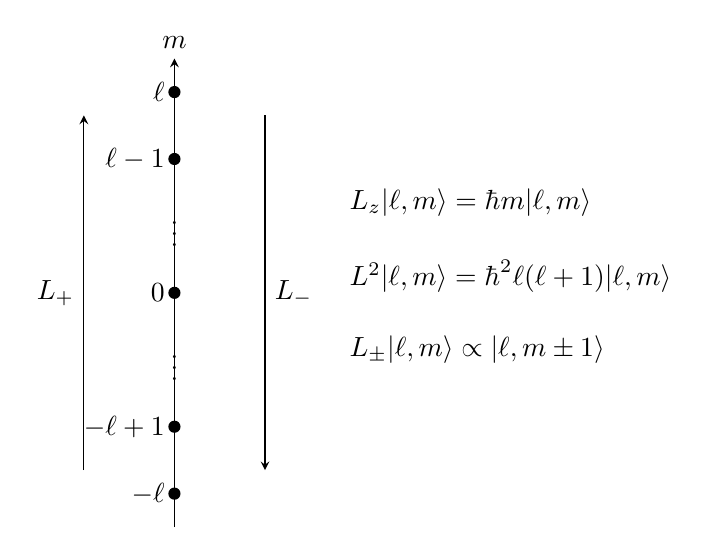
\begin{tikzpicture}[x=1cm,y=0.85cm,>=stealth]
\draw[->] (0,-3.5) -- (0,3.5) node[above] {$m$};

\fill (0,3) circle (2.2pt);
\fill (0,2) circle (2.2pt);
\fill (0,0) circle (2.2pt);
\fill (0,-2) circle (2.2pt);
\fill (0,-3) circle (2.2pt);

\node[left] at (0,3) {$\ell$};
\node[left] at (0,2) {$\ell-1$};
\node[left] at (0,0) {$0$};
\node[left] at (0,-2) {$-\ell+1$};
\node[left] at (0,-3) {$-\ell$};

\node at (0,1) {$\vdots$};
\node at (0,-1) {$\vdots$};

\draw[->] (-1.15,-2.65) -- (-1.15,2.65)
node[midway,left] {$L_+$};
\draw[->] (1.15,2.65) -- (1.15,-2.65)
node[midway,right] {$L_-$};

\node[anchor=west] at (2.1,1.35)
{$L_z|\ell,m\rangle=\hbar m|\ell,m\rangle$};
\node[anchor=west] at (2.1,0.25)
{$L^2|\ell,m\rangle=\hbar^2\ell(\ell+1)|\ell,m\rangle$};
\node[anchor=west] at (2.1,-0.85)
{$L_\pm|\ell,m\rangle\propto|\ell,m\pm1\rangle$};
\end{tikzpicture}
\caption{整数の軌道角運動量多重項。\(L_+\)と\(L_-\)は\(m\)を1だけ変えるが、\(L^2\)は多重項全体を通して\(\hbar^2\ell(\ell+1)\)のままである。}
\lectureframe{00:35:53}
\end{figure}

\section{中心力問題}

次を考える。
\begin{equation}
H=\frac{\mathbf p^2}{2m}+V(r),
\end{equation}
ここで\(V\)は原点からの距離のみに依存する。回転対称性は角運動量の保存を意味する。古典的には、\(\mathbf L\)は大きさと向きが固定されているので、軌道は\(\mathbf L\)に垂直な平面内にとどまる。軌道は円形である必要も、閉じている必要もない。

この古典的軌道面が\(xy\)平面になるように座標を選び、運動量を動径成分と接線成分に分解する。
\begin{equation}
\mathbf p^2=p_r^2+p_\theta^2.
\end{equation}
角運動量の大きさは
\begin{equation}
L=r p_\theta,
\end{equation}
であるから、接線成分への寄与は
\begin{equation}
p_\theta^2=\frac{L^2}{r^2}.
\end{equation}
と書ける。ハミルトニアンは
\begin{equation}
H=\frac{p_r^2}{2m}+\frac{L^2}{2mr^2}+V(r).
\end{equation}
となる。\(L\)を固定すると、これは動径座標における一次元問題であり、有効ポテンシャルは
\begin{equation}
V_{\mathrm{eff}}(r)=\frac{L^2}{2mr^2}+V(r).
\end{equation}
である。動径ハミルトニアンは下の黒板に示されている。\footnote{ソースフレーム：\texttt{\detokenize{lecture_03_frame_02.png}}、講義動画\(00{:}47{:}15\)。}

\begin{figure}[htbp]
\centering
\includegraphics[width=0.9\linewidth]{lecture_03_frame_02.png}
\caption{固定された古典的角運動量に対して、動径ハミルトニアンは動径運動エネルギー、遠心項\(L^2/(2mr^2)\)、および中心ポテンシャル\(V(r)\)を含む。}
\lectureframe{00:47:15}
\end{figure}

\(1/r^2\)項は遠心障壁である。粒子が原点に近づくにつれて増大するので、対応する力は外向きである。ここで議論しているクーロン型の引力に対しては、\(L\neq0\)である軌道は中心に到達する代わりに中心の周りを回る。\(L=0\)のとき、障壁は存在しない。

引力クーロンポテンシャル
\begin{equation}
V(r)=-\frac{\kappa}{r},
\end{equation}
に対して、遠心項は小さい\(r\)で支配的であり、一方クーロン項はよりゆっくり減少し、大きい\(r\)で支配的である。\(L\neq0\)に対して、それらの和は極小をもつ。極小における運動は半径が一定であり、したがって円運動である。極小より上で脱出閾値より下の束縛運動は、最小半径と最大半径の間で振動する。クーロン問題では、これらは楕円軌道の動径振動である。

\section{換算動径方程式}

量子力学では、確定した軌道角運動量をもつ状態の角度部分は球面調和関数である。分離された状態を
\begin{equation}
\Psi_{n_r\ell m}(r,\theta,\phi)
=\frac{u_{n_r\ell}(r)}{r}\,
Y_{\ell m}(\theta,\phi).
\end{equation}
と書く。角度演算子\(L^2\)は固有値
\begin{equation}
L^2Y_{\ell m}
=\hbar^2\ell(\ell+1)Y_{\ell m}.
\end{equation}
をもつ。固定された組\(n_r,\ell\)に対して、\(u_{n_r\ell}(r)\)を\(u(r)\)と略記する。換算動径関数に対して残る方程式は
\begin{equation}
\begin{aligned}
&-\frac{\hbar^2}{2m}\frac{d^2u}{dr^2}
+\frac{\hbar^2\ell(\ell+1)}{2mr^2}u(r)\\
&\qquad+V(r)u(r)=E_{n_r\ell}\,u(r).
\end{aligned}
\end{equation}
である。

\editorialnote{純粋な一次元二階微分方程式は換算動径関数\(u=rR\)を用いる。したがって、表示された講義の方程式における\(\psi(r)\)は\(u(r)\)に対応し、一方\(\Psi=R(r)Y_{\ell m}\)における通常の動径因子は\(R=u/r\)である。この規約は、\(-i\hbar\,d/dr\)を三次元動径ヒルベルト空間上の独立したエルミート動径運動量演算子として扱うことを避ける。}

換算動径方程式は下の黒板に示されている。\footnote{ソースフレーム：\texttt{\detokenize{lecture_03_frame_03.png}}、講義動画\(00{:}54{:}32\)。}

\begin{figure}[htbp]
\centering
\includegraphics[width=0.9\linewidth]{lecture_03_frame_03.png}
\caption{固定された\(\ell\)に対して、換算動径波動関数は、\(\ell(\ell+1)/r^2\)に比例する遠心項をもつ一次元のSchr\"odinger方程式を満たす。}
\lectureframe{00:54:32}
\end{figure}


三次元の角度構造はパラメータ\(\ell\)に圧縮された。磁気量子数\(m\)は動径方程式に現れない。

\begin{classroomqa}
\lecturetimestamp{00:55:34}
\audiencequestion{与えられた\(\ell\)に対して、\(2\ell+1\)個の磁気状態は同じエネルギーをもつか。}
\lecturerresponse{はい、動径固有状態も固定されている場合には。選ばれた各\(u_{n_r\ell}\)に対して、すべての値\(m=-\ell,\ldots,\ell\)は同じエネルギーをもつ。なぜなら\(m\)は動径方程式に入らないからである。同じ\(\ell\)における異なる動径固有状態は一般に異なるエネルギーをもつ。}
\end{classroomqa}

\begin{classroomqa}
\lecturetimestamp{00:56:03}
\audiencequestion{なぜ\(L^2\)を\(\hbar^2\ell(\ell+1)\)で置き換えてよいのか、また\(\ell\)は\(m\)の許される値とどのように関係するのか。}
\lecturerresponse{数\(\ell\)は角運動量多重項をラベルし、その最大の\(m\)値である。その多重項のすべての状態は同じ\(L^2\)固有値\(\hbar^2\ell(\ell+1)\)をもつので、その固有値が動径方程式に代入される。}
\end{classroomqa}

明示的な特殊関数解は現在の議論には必要ない。重要なのは解がどのように組織されるかである。

\section{動径ノードとエネルギー準位}

固定された\(\ell\)に対し、換算動径方程式は通常の一次元固有値問題である。その束縛状態は内部ノードの数によって順序づけられる。最も低い動径状態は内部ノードをもたず、次は一つ、その次は二つもつ。ノードが多いほど波動関数の変化は速くなり、変化が速いほど運動量は大きくなり、したがって運動エネルギーも大きくなる。

\(\ell\)の各値は、遠心項が\(\ell\)とともに変化するため、異なる動径演算子を定義する。したがって\(\ell=0,1,2,\ldots\)は別々の動径の塔を与える。正の遠心項は、角運動量が加わるにつれて準位を上方へずらす。固定された\(\ell\)における各動径固有値は、次元
\begin{equation}
2\ell+1.
\end{equation}
の磁気多重項を担う。\(\ell=0\)準位は一重項、\(\ell=1\)準位は三重項、\(\ell=2\)準位は五重項である。これらは回転対称性によって保証される縮退である。付加的な対称性により、異なる\(\ell\)値をもつ状態も縮退しうる。

大きな\(r\)で\(V(r)\to0\)を満たす原子型ポテンシャルに対し、脱出閾値は慣例的に\(E=0\)である。負エネルギーの状態は離散束縛スペクトルをなす。\(E=0\)以上では散乱連続状態に出会う。この記述はポテンシャルの大きな\(r\)での振る舞いに依存し、閉じ込め型中心ポテンシャルには当てはまらない。

\section{特別なクーロン縮退}

厳密な非相対論的クーロンポテンシャルには、準位の付加的な整列がある。最も低い\(\ell=1\)動径状態は、第一励起\(\ell=0\)状態と同じエネルギーをもつ。次の\(\ell=1\)状態は第二励起\(\ell=0\)状態と整列し、最も低い\(\ell=2\)状態がそれらに加わる。このパターンはより高い動径および角運動量の塔へと続く。

\begin{classroomqa}
\lecturetimestamp{01:09:57}
\audiencequestion{この余分なクーロン縮退は別の対称性を示すのか。}
\lecturerresponse{はい。それは厳密なクーロンポテンシャルの異常な付加的対称性である。ポテンシャルの小さな変化はこの整列を壊し、その導出はここでは追わない。}
\end{classroomqa}

その結果得られる軌道殻の縮退は
\begin{equation}
1,\qquad 4,\qquad 9,\qquad 16,\qquad \ldots
\end{equation}
であり、電子スピンを含める前のものである。

\begin{classroomqa}
\lecturetimestamp{01:11:46}
\audiencequestion{この縮退は水素を記述するのか、それとも理想的なクーロン問題のみを記述するのか。}
\lecturerresponse{水素はそれを非常に良い近似で満たすが、厳密にではない。相対論的補正と原子核の有限な大きさが理想的なクーロンのパターンを乱す。}
\end{classroomqa}

点状原子核は厳密な\(1/r\)ポテンシャルを生じる。電荷が小さな体積に広がった原子核は、電子がその体積に侵入するときわずかに異なるポテンシャルを生じ、このわずかなずれでさえ特別な縮退の一部を解消する。

スピンも省略されている。二つの電子スピン状態を含めると、殻の数は
\begin{equation}
2,\qquad 8,\qquad 18,\qquad 32,\qquad \ldots
\end{equation}
に倍増する。これは、より完全な原子の取り扱いにおけるさらなる分裂が分解される前のものである。

\section{デカルト方程式再訪}

動径問題が出発した方程式は、三次元の時間に依存しないSchr\"odinger方程式
\begin{equation}
\begin{aligned}
-\frac{\hbar^2}{2m}\nabla^2\Psi+V(r)\Psi&=E\Psi,\\
\nabla^2&=\frac{\partial^2}{\partial x^2}
+\frac{\partial^2}{\partial y^2}
+\frac{\partial^2}{\partial z^2},\\
r&=\sqrt{x^2+y^2+z^2}.
\end{aligned}
\end{equation}
である。動径座標と角度座標へ移り、\(L^2\)の固有状態を選ぶ。次に\(L^2\)を\(\hbar^2\ell(\ell+1)\)で置き換えると、偏微分方程式は上記の通常の動径方程式に帰着する。

\begin{classroomqa}
\lecturetimestamp{01:16:42}
\audiencequestion{理想的なクーロンスペクトルからのずれを原子核の大きさの決定に用いることができるか。}
\lecturerresponse{この単純な比較ではできない。他の補正の方がはるかに大きく、まずそれらを考慮に入れなければならない。原子核の大きさをここで挙げたのは、点状クーロンポテンシャルからのずれの即座の例を与えるからである。}
\end{classroomqa}

\begin{classroomqa}
\lecturetimestamp{01:17:09}
\audiencequestion{古典的な角運動量の項と量子力学的な角運動量の項の主な違いは何ですか。}
\lecturerresponse{古典的には \(L^2\) は保存されたベクトルの大きさの通常の二乗である。量子力学的な軌道多重項では、その固有値は \(\hbar^2\ell(\ell+1)\) であり、単に \(\hbar^2\ell^2\) ではない。付加的な項は角運動量の成分が非可換であることに由来する。}
\end{classroomqa}

\begin{classroomqa}
\lecturetimestamp{01:17:58}
\audiencequestion{束縛状態の波動関数はコンパクトな台を持つか。}
\lecturerresponse{いいえ。それらは中心から任意に遠くまで広がる。ここで議論している原子の束縛状態では、大きな距離で指数関数的に減少するので、確率は無視できるほど小さくなるが、有限の半径を超えて消えるわけではない。}
\end{classroomqa}

\begin{classroomqa}
\lecturetimestamp{01:18:48}
\audiencequestion{\(\ell=0\) が遠心井戸を取り除くと、安定点はどうなるか。}
\lecturerresponse{遠心障壁と引力の競合によって生じる極小はもはや存在しない。点クーロンの理想化では、古典的運動は特異な中心へ向かう。量子力学的には、最低状態が中心に正確に確定した位置とゼロの運動量を同時に持つことはできないので、最低波動関数は有限の空間的広がりを持つ。}
\end{classroomqa}

\editorialnote{正則な中心ポテンシャルに対しては、古典的な角運動量ゼロの軌道は原点を通り抜けて続くことがある。理想的な点クーロンポテンシャルでは、代わりに \(r=0\) が衝突特異点であり、古典的軌道の継続には追加の処方則が必要である。}

古典的な簡約は単一の軌道を平面内に置いたが、その手順を量子力学的波動関数に同じようには適用できない。量子力学的な軌道状態は三次元空間を満たす。完全な角運動量演算子は \(L^2=L_x^2+L_y^2+L_z^2\) であり、その固有値は三次元の結果 \(\hbar^2\ell(\ell+1)\) を保つ。

\begin{classroomqa}
\lecturetimestamp{01:21:30}
\audiencequestion{古典的軌道が平面内に置かれた後、なぜ量子力学的問題は三次元のままであり得るのか。}
\lecturerresponse{保存された角運動量ベクトルに垂直な座標を選ぶことによって固定平面内に置かれたのは古典的軌道だけである。量子力学的波動関数は三次元空間を占める。他の角運動量成分は \(L^2\) を通じて依然として存在しており、そのため動径方程式には一つの成分の二乗だけではなく \(\ell(\ell+1)\) が含まれる。}
\end{classroomqa}

\begin{classroomqa}
\lecturetimestamp{01:22:54}
\audiencequestion{すべての量子力学的問題が昇降演算子を持つか。}
\lecturerresponse{いいえ。それらは異常に好都合な場合に現れる。角運動量はその一例であり、調和振動子もまた別の例である。振動子の場合が特に有用なのは、安定平衡近傍の運動が、有効ポテンシャルの極小近傍での小さな動径振動を含めて、しばしば近似的に調和振動となるからである。}
\end{classroomqa}

この時点で原子の問題は脇に置かれ、調和振動子がはしご演算子によって決定されるスペクトルの次の例となる。

\section{小さな振動と調和振動子}

安定平衡の近傍では、十分に小さな変位はしばしば調和振動を生じる。角運動量が非零の場合の有効動径ポテンシャルが一例を与える。すなわち、その井戸の底に近い動径運動は近似的に調和振動である。

単位質量の一次元振動子を考える。\(x\) を平衡からの変位とし、ばね定数を \(k=\omega^2\) と書く。古典的ハミルトニアンは
\begin{equation}
H=\frac{p^2}{2}+\frac{\omega^2x^2}{2}.
\end{equation}
である。ハミルトンの方程式は
\begin{equation}
\dot{x}=\frac{\partial H}{\partial p}=p,
\qquad
\dot{p}=-\frac{\partial H}{\partial x}=-\omega^2x,
\end{equation}
を与え、したがって
\begin{equation}
\ddot{x}=-\omega^2x.
\end{equation}
となる。ゆえに \(\omega\) は古典的振動数である。

\section{因数分解と零点エネルギー}

量子力学的には、
\begin{equation}
[x,p]=i\hbar.
\end{equation}
である。ハミルトニアンは二乗の和であり、因数分解
\begin{align}
\frac{1}{2}(p+i\omega x)(p-i\omega x)
&=\frac{1}{2}\left(p^2+\omega^2x^2+i\omega[x,p]\right) \\
&=\frac{1}{2}\left(p^2+\omega^2x^2-\hbar\omega\right).
\end{align}
を示唆する。したがって
\begin{equation}
H=\frac{1}{2}(p+i\omega x)(p-i\omega x)
+\frac{1}{2}\hbar\omega.
\end{equation}
となる。付加的な項 \(\hbar\omega/2\) は零点エネルギーである。

古典的には最低エネルギーは \(x=p=0\) で生じるであろう。量子力学的には、位置と運動量の両方がゼロに鋭く固定された状態は存在し得ない。さらに、二つの項 \(p^2/2\) と \(\omega^2x^2/2\) は正であり、相殺することはできない。したがって非零の基底状態エネルギーは避けられない。

はしごの計算では、共通の付加定数は一時的に脇に置き、最後に復元してよい。

\begin{classroomqa}
\lecturetimestamp{01:36:10}
\audiencequestion{零点の項が正であることは、さらに何かを教えてくれるか。}
\lecturerresponse{振動子のハミルトニアンは正の演算子である。すなわち正の二乗の和であるから、そのエネルギーは負にはなり得ない。}
\end{classroomqa}

\section{振動子のはしご}

無次元演算子\footnote{を導入する。\(01{:}37\)--\(01{:}42\)の周辺では、計算は\(\hbar=1\)を用いる。\(\hbar\)の因子は、\(A_\pm\)が無次元となり、その交換子が1となるように、これらの規格化された定義において復元される。}
\begin{equation}
A_+=\frac{p+i\omega x}{\sqrt{2\hbar\omega}},
\qquad
A_-=\frac{p-i\omega x}{\sqrt{2\hbar\omega}}.
\end{equation}
これらはエルミート共役である：
\begin{equation}
A_+^\dagger=A_-.
\end{equation}
それらの交換子は
\begin{align}
[A_-,A_+]
&=\frac{1}{2\hbar\omega}
\left([p,i\omega x]+[-i\omega x,p]\right) \\
&=1.
\end{align}

定義する
\begin{equation}
N=A_+A_-.
\end{equation}
このときハミルトニアンは
\begin{equation}
H=\hbar\omega\left(N+\frac{1}{2}\right).
\end{equation}
したがって、エネルギー準スペクトルを見つけることは\(N\)の固有値を見つけることに帰着する。

仮定する
\begin{equation}
N|n\rangle=n|n\rangle.
\end{equation}
\(N\)との交換子は\footnote{\(01{:}45{:}37\)--\(01{:}48{:}10\)における中間段階は、述べられた関係\(N=A_+A_-\)および\([A_-,A_+]=1\)から直接再構成される。}
\begin{align}
[N,A_+]
&=A_+[A_-,A_+]=A_+, \\
[N,A_-]
&=[A_+,A_-]A_-=-A_-.
\end{align}
したがって
\begin{align}
N\bigl(A_+|n\rangle\bigr)
&=(n+1)A_+|n\rangle, \\
N\bigl(A_-|n\rangle\bigr)
&=(n-1)A_-|n\rangle.
\end{align}
ゆえに、\(A_+\)は\(N\)の固有値を1だけ上げ、\(A_-\)は、結果として得られるベクトルが非零であるときはいつでも、それを1だけ下げる。

演算子\(N\)は非負である：
\begin{equation}
\langle\psi|N|\psi\rangle
=\langle\psi|A_+A_-|\psi\rangle
=\|A_-|\psi\rangle\|^2
\geq0.
\end{equation}
したがって、下降過程は負の固有値へと続くことはできない。底状態\(|b\rangle\)において、それは終了しなければならない：
\begin{equation}
A_-|b\rangle=0.
\end{equation}

規格化された固有状態に対して、はしごの係数はそれらのノルムによって固定される：
\begin{align}
\|A_-|n\rangle\|^2
&=\langle n|A_+A_-|n\rangle=n, \\
\|A_+|n\rangle\|^2
&=\langle n|A_-A_+|n\rangle=n+1.
\end{align}
したがって、位相は次のように選ばれ得る：
\begin{equation}
A_-|n\rangle=\sqrt{n}\,|n-1\rangle,
\qquad
A_+|n\rangle=\sqrt{n+1}\,|n+1\rangle.
\end{equation}

\begin{classroomqa}
\lecturetimestamp{01:52:42}
\audiencequestion{もし\(A_-\)が状態を下げ、\(A_+\)がそれを再び上げるなら、\(A_+A_-\)はどのようにして固有値\(n\)を生み出すのか？}
\lecturerresponse{はしごの作用には規格化因子が含まれる。まず\(A_-\)を作用させると\(\sqrt n\)が寄与し、結果として得られる状態に\(A_+\)を作用させるとさらに\(\sqrt n\)が寄与する。それらの積は\(n\)である。}
\end{classroomqa}

確かに、
\begin{equation}
A_+A_-|n\rangle
=\sqrt n\,A_+|n-1\rangle
=n|n\rangle.
\end{equation}

\begin{classroomqa}
\lecturetimestamp{01:55:52}
\audiencequestion{\(N\)の最低固有値はゼロでなければならないのか、それとも正であり得るのか？}
\lecturerresponse{それはゼロでなければならず、\(N\)のスペクトルは非負整数からなる。端点の証明はまだ与えられていない。}
\end{classroomqa}

\editorialnote{\(|b\rangle\)を最低状態とする。下降は終了しなければならないので、\(A_-|b\rangle=0\)。直ちに\(N|b\rangle=A_+A_-|b\rangle=0\)が従い、したがって\(N\)の最低固有値はゼロである。}

この最低状態から出発して\(A_+\)を作用させると
\begin{equation}
n=0,1,2,\ldots.
\end{equation}
加法的な零点項を復元すると、振動子のエネルギーは
\begin{equation}
E_n=\hbar\omega\left(n+\frac{1}{2}\right),
\qquad n=0,1,2,\ldots.
\end{equation}

振動子代数はさらに発展させられ、他の量子問題を解くために用いられる。
